% which shows that the imposed conditions are necessary for the problem. 

% For convenience reasons, we leave the {\it overlapping} form of arbitrage and study it in the form of Fig.~\ref{fig:sep-arb} in which the exploiter of each arbitrage needs to fulfill his principals, i.e. in the case of using "any one can pay" \ahC{Footnote?}, by connecting the output of exercise transaction from previous swaption. However, Applying the ideas to this section on the form of Fig.\ref{fig:overlap-arb} is straightforward.
% then
% after giving some definitions of the problem domain we suggest some conditions on our problem. Afterward we give a constructive proof to show that the imposed conditions are necessary to settle the case.


% \melikaC{behtar nist nagim "we leave the overlapping form"? chon in graphe model sazi shode hamooneh.}

% \ahC{We have to mention that we avoid considering multi output swaptions}

    
    % Each node of the graph is dedicated to a swaption. The right hand side name inside each node is the name of the swaption {\it Owner}. A color is dedicated to each party. A node is colored by the color of its {\it Owner}. An arc represents transfer of principal between two swaptions. Each arc is colored by the color of the party whose principal is being transferred between its corresponding swaptions (In behalf of using the {\it Overlapping } technique). An example of this graph is presented in Fig.~\ref{fig:gen-graph}.
    % is defined to show whether an edge is internal or external or  to swaptions.
    
    
    % For each $e \in E$, if $\tau(e)=i$, . If $\tau(e)=x$, 
    % In this graph 
    
    % \fatemeC{In this graph, each swaption is pictured as two nodes encapsulated in a rectangle, each node representing one of the parties. In practice the external arcs are replaced with the overlapping technique and neighbour swaptions are merged into one.} 
    
    
    % In this graph, 
    
    % $opposite(head(e))=v$, then successor(v) = $tail(e)$ 
    % It is clear that for each $e$ that $\tau(e) = ex$, $label(opposite(tail(e))) = label(head(e))$, 
    
    % if there is a black arc between two swaptions, then in the source swaption, the label of the node other than the head of the black arc is the same as the label of the tail node of this arc, 
    
    % in the source swaption the node other than arc's head
    
    
    
    
    % \item \textbf{\keyoneGraphExtended graph}: 
    
    % In this graph we extend the \keyoneGraph graph by adding new dashed-line arcs between two swaptions. The algorithm for drawing these arcs is as follows:
    % \begin{enumerate}
        % \item set $\mathcal{S} = \{s_0,\ ,s_1, ..,\ s_n\}$ the set of nodes in the \keyoneGraph graph which does not have any ingoing black arc.
    %     \item for $i$ in $(0,\ n)$:
    %     \item \tab set $ns$ equal to the $s_i$;
    %     % \item \tab set $sw$ equal to the swaption in which $ns$ is located;
    %     \item \tab set $os$ equal to the other node than $ns$ in its \tab swaption;
    %     \item \tab while $os$ has an outgoing black arc:
    %     \item \tab \tab set $ns$ equal to the destination node of \tab\tab the black arc;
    %     \item \tab \tab set $os$ equal to the other node than \tab\tab $ns$ in its swaption;
    %     \item \tab \tab draw a new dashed-arc originating from \tab\tab $os$ and destined to $s_i$;
    % \end{enumerate} \ahC{Figure is neededddd, also change the other figures to match with this one}
    % Note that in this graph, we name the dashed-arc and red arcs the \textbf{Reversible} arcs of the graph.
    % \item \textbf{\AtwoGraph Graph}: This graph shows the order of keys imposition (both \Atwo and \Aone keys) on swaptions. Same as \keyoneGraph graph, each node on this graph also represents a swaption. The red arcs inside each swaption is originated from the swaption {\it Owner} and destined to the other party (From right to left). The black arcs between swaptions follows the order of principals flow.
% \end{enumerate}
% \ahC{Mention in the swaption section that late deposition is jeddan geron tar az early depositione}


% The main assumption beneath our case study is the parties rationality. The required rationality property is as follows:

% \begin{assumption}
% \label{assumption:rationality}
% Since the premium of a late deposition swaption is significantly more expensive than the premium in a early deposition one, a party $p$ is rational if:
% \begin{enumerate}
%     \item When she owns enough value to buy an {\it Early Deposit} \ie she can deposit her principal earlier than the other one, she does not buy a {\it Late Deposit} one.
    
%     \item When she owns enough value to sell a {\it Late Deposit} swaption \ie she can deposit her principal earlier than the other one, she does not sell a {\it Late Deposit} one.
% \end{enumerate}

% % and if she wants to deposit the needed principal by her own, she can change the type of the swaption 
% \end{assumption}

% \begin{definition}
% {\it Concurrent Protocol}\\
% An Atomic Cross-chain Swaption Protocol $P$ is consists of signing and sending on chain all the transactions of a tangle in a specific order. We define a protocol is Concurrent if the signing and sending steps are completely ran separately and in its procedure no transaction broadcasting occur before any other transaction signing.
% \end{definition}

% Later we will refer to these stages as \textbf{Contract Settlement} and \textbf{Contract Initiation}.

% To give the definitions about flow of principal through the tangle first we need to design a new graph
% the association set of a party $p$ is the set of vertices $U$ which $p$ is one of the participated parties in.
% \fatemeC{define owner if it is not defined}
% In the scope of Theorem~\ref{th:concurrency} only one unique party is acceptable to decide whether she wants the entire tangle to be exercised or not (in fact, expose the \Atwo key of the entire tangle or not). Hence, she can cheat. So, we have to prevent this party from cheating on others by stealing their premium in other swaptions, since this party may pretend herself someone else in other swaptions with other parties. To do so, we assume that the main owner has to pay other parties premium more than the summation of the premiums each of them has to pay for their own swaptions.
% We call the initial premium of a party $p$, the \textbf{feeding premium} of him and the swaption in which he gets his initial premium, the \textbf{genesis} swaption of this party. In the $GG$ graph, we define the function $genesis: P\to V$ and reference to this swaption as $genesis(p)$.
% It is like the situation that in every swaption the main owner is acting as the swaption owner even if this position is not marked by her label. Through the rest of this section, we leave this transition while keeping in mind that the main owner of tangle can not cheat on others this way. \fatemeC{severe edit needed} 

 
% We reference to the genesis swaption of party $p$ using $genesis(p)$


% To continue the proof, we need to figure out which party will be the owner of tangle. For finding this party we design the below algorithm: 


% we design a multiple partial tournament $tour$ in which every vertices in $GG$ graph represents a match in $tour$, then execute the below algorithm:
% \begin{lstlisting}
% Set \mathrm{$\mathcal{C}=\{c_1,\ c_2,\ .., c_n\}$}
% For $i \in $
% \end{lstlisting}
% A party $p$ can be an eligible winner if for every other eligible winner $e$ there is a series of matches in which $e$ wins $p$, then there is another series of match in with $p$ also wins over $e$ directly or indirectly. 
% In the beginning of the algorithm all the parties are eligible candidates.
% An eligible winner $e$ if for every other eligible winner there is a series of match in which is who has won all other parties directly or indirectly through the series of matches.
% Given a \genGraph graph of concurrent tangle $T$, for each vertex do the following line:\\
% Replace the left hand side label on the node through the entire graph with the label appeared in the right hand side.
% The algorithm has at least one output, because the loop finally will be stopped when the list of eligible candidates has one party.
% The output of the {\it Owner Finder} algorithm may not be unique depends on the order of nodes are being processed. This algorithm only give the list of all candidate l

% \begin{definition}
% A concurrent tangle $T$ has owner if at least one of the candidate parties in the output of algorithm~\ref{algo:owner-finder} on $T$ has a mother vertex in the \genGraph graph of $T$. We call this party interchangeably the {\it Owner} of $T$ or the \Atwo key holder of $T$.
% A concurrent tangle $T$ has owner if after the execution of algorithm~\ref{algo:owner-finder} on $T$, all of the labels on each vertexes are the same. We call the party corresponding to this label the {\it Owner} of $T$. Interchangeably we call the Owner \Atwo Key Holder of $T$ also.
% \end{definition}
% if output of the execution of the algorithm~\ref{algo:owner-finder} on $T$ 
% A concurrent tangle $T$ is \AtwoGraph Acceptable if at least one of the candidate parties on the output of algorithm~\ref{algo:owner-finder} has a mother vertex in the \genGraph graph of $T$. 
% We also name the swaption corresponding to this Mother vertex the genesis swaption of $T$.
% \begin{definition}{\keyoneGraph acceptable}\\
% A concurrent tangle $T$ is \keyoneGraph acceptable if its \keyoneGraph graph is a directed acyclic graph with only one source. We call the party corresponding to this unique source the \keyone key holder. 
% \end{definition}
% \begin{definition}{nemidonam che esmi}\\
% A concurrent tangle $T$ is {nemidonam che esmi} Acceptable if the subgraph $SG=(\hat{V}, \hat{E})$ of $PFG=(V, E)$ where $\hat{V}=V$ and $\hat{E} = \{e \in E | \tau(e) \neq t\}$ is a DAG with one source and $PFG$.
% \end{definition}


% \begin{definition}{\it Insecure Cycle}\\
% A cycle $\mathcal{C}$ is insecure if $\nexists_{e\ \in \ \mathcal{C}}$ where $e$ is reversible or if $\exists_{e\ \in \ \mathcal{C}}$ where $e$ is reversible then $label(tail(e)) \neq$ key holder's label.
% A cycle $\mathcal{C}$ is insecure if $\exists_{e\ \in \ \mathcal{C}}$ where $e$ is reversible and $label(tail(e)) \ne$  \keyone key holder.
% \end{definition}
% Assume $$
% A concurrent tangle $T$ is \keyoneGraph acceptable if there is no insecure cycle in its \keyoneGraph graph, and this graph has only one source. We call this source, the \depsrc of $T$.
% $SG=(\hat{V}, \hat{E})$ of $PFG=(V, E)$ where $\hat{V}=V$ and $\hat{E} = \{e \in E | \tau(e) = x\}$ and subgraph

% \begin{definition}{\it \depsrc}\\
% In a \keyoneGraph acceptable tangle, we call the swaption in  which the source is located on the \keyoneGraph graph the \depsrc swaption of the tangle.
% \end{definition}




% \begin{definition}{\it \keyoneGraph Acceptable}\\
% Given a concurrent tangle $T$, assume $\mathcal{S}=\{s_1,\ s_2,\ ..,\ s_n\}$ is the set of sink nodes in the \keyoneGraph graph of $T$ and in $\mathcal{SW}=\{sw_1,\ sw_2,\ ..,\ sw_n\}$ every $sw_i$ references to the swaption in which $s_i$ is one of its nodes. We call $T$ is \keyoneGraph Acceptable if its \keyoneGraph graph is a directed acyclic graph with one source and for every $sw_i$ the node other than $s_i$ belongs to the unique source of graph. In the other words, the other node in all the $sw_i$s are labeled with the label of the party whose node is the source of the graph. We also call the swaption in which the source is located the \depsrc swaption of the tangle.
% the label of the party whose nodes is the source of the graph 
% and the parties in front of all of the elements of $\mathcal{S}$ in their swaptions 
% A concurrent tangle is \keyoneGraph Acceptable if its representation in \keyoneGraph graph is a directed acyclic graph with one source and the the parties corresponding to the other node in the swaptions which contain sink nodes are the same with the party who is the unique source. We call the swaption in which this source is located the \depsrc swaption of the tangle.
% \end{definition}
% \begin{definition}{\it Loop Owner}
% A loop of swaptions might has a loop owner if the {\it owner} of all of the swaptions are the same party.
% \end{definition}

% \begin{definition}{Mother Vertex}\\
% In a graph, a Mother Vertex $v$ is a vertex such that for every other vertexes in the graph $\hat{v}$, there is a path beginning from $v$ and ends to $\hat{v}$.
% \end{definition}

% \begin{corollary}
% \label{cor:mother}
% Given a graph $G$, assume the Mother vertexes are $M = \{m_1, m_2, .., m_n\}$. For all $m_i\ and\ m_j \in  M$ there is a loop $l$, and all of the vertexes in $l$ are in $M$.
% % between each two Mother Vertexes there is a loop which its vertexes are all Mother's $v$ is a vertex such that for every other vertexes in the graph, there is a path beginning from $v$.
% \end{corollary}


% A tangle $T$ is \AtwoGraph Acceptable if it has a unique Owner and there exists a Mother vertex on \AtwoGraph graph of $T$ which has the same label as the Owner of the $T$. We name the swaption corresponding to this Mother vertex the genesis swaption of $T$.

% In a Concurrent tangle $T$, if after executing algorithm~\ref{algo:owner-finder} on $T$ all of the labels are the same
% the label of all of the Mother vertexes in $T$ are the same, then we call the tangle $T$ is \AtwoGraph Acceptable. We call the party corresponding to this label the {\it Owner} of $T$.

% A concurrent tangle is \AtwoGraph Acceptable if its representation in \AtwoGraph graph form only and only contains one loop in which every swaptions participating in the loop has the same owner. We call the so called loop the {\it Main Loop} or {\it Main Arbitrage} of the tangle.

% After executing the above algorithm, 

% \begin{definition}{\it \Atwo Key Holder}
% In a \AtwoGraph Acceptable concurrent tangle, the label of its Mother vertexes is called \Atwo Key Holder.
% \end{definition}

% \begin{definition}{\it \AtwoGraph Acceptable}
% % Given a concurrent tangle $T$, assume $\{l_0, l_1, .., l_n\}$ are the loops in representation of $T$ in \AtwoGraph graph form in which every swaptions participating in the loop has the same owner. The $T$ tangle is \AtwoGraph Acceptable if the owner of $l_i$s are the same party.

% In a Concurrent tangle $T$, if the label of all of the Mother vertexes in $T$ are the same, then we call the tangle $T$ is \AtwoGraph Acceptable. We call the party corresponding to this label the {\it Owner} of $T$.

% % A concurrent tangle is \AtwoGraph Acceptable if its representation in \AtwoGraph graph form only and only contains one loop in which every swaptions participating in the loop has the same owner. We call the so called loop the {\it Main Loop} or {\it Main Arbitrage} of the tangle.
% \end{definition}



% \begin{corollary}
% \label{cor:mother-2}
% Using the result of the corollary~\ref{cor:mother}, we can conclude that in a {\it \AtwoGraph Acceptable} tangle if there is more than one Mother vertex, then there is at least one loop in its \AtwoGraph graph form which consists of Mother vertexes in the tangle.
% \end{corollary}

% Assume the {\it \AtwoGraph Acceptable} tangle $T$ which has more than one Mother vertex. By the result of \ref{cor:mother-2} we know that there is a loop in \AtwoGraph graph of $T$ which the owner of its swaptions are all the $T$ owner. We can say that this loop also exists in \keyoneGraph graph of $T$ if the swaptions of the loop all has red arcs from right to left. Hence $T$ is no longer {\it \keyoneGraph Acceptable}. Using this argument we can conclude the following theorem:

% \begin{theorem}
% In a Concurrent Executable tangle $T$, there is at least a swaption between $T$'s Mother vertexes which its red arc in the \keyoneGraph graph form is from left to right. We call this swaption the Genesis Swaption of $T$. Genesis swaption is supposed to be the first one which is processed in the arbitrage.
% \end{theorem}

% \begin{definition}{\it Genesis Swaption}
% In a concurrent tangle, the swaption in which \Atwo key holder and \keyone key holder are faced together is called the Genesis Swaption. This swaption is supposed to be the first one which is processed in the arbitrage. 
% \end{definition}
% \begin{definition}{\it Startable}
% A concurrent tangle is Startable if it has a Genesis Swaption, and the \keyone key holder and the \Atwo key holder of the swaption are the same as the \keyone key holder and the \Atwo key holder in the tangle respectively.
% \end{definition}




% \begin{definition}{\it Genesis Swaption}
% In a \keyoneGraph Acceptable tangle, the swaption in which \keyone Key Holder is located on is called the Genesis Swaption. This swaption is supposed to be the first one which is processed in the arbitrage. 
% \end{definition}

% \begin{definition}{\it Genesis Swaption}
% Given a \AtwoGraph Acceptable tangle $T$, assume $\{s_1, s_2, .., s_n\} $ is the set of swaptions in which \Atwo Key Holder is their owners. If there exists a $s_i$ which its red arc in \keyoneGraph is from left to right, then $s_i$ is the Genesis Swaption of $T$. Otherwise 
% In a \keyoneGraph Acceptable tangle, the swaption in which \keyone Key Holder is located on is called the Genesis Swaption. This swaption is supposed to be the first one which is processed in the arbitrage. 
% \end{definition}


% \subsubsection{Security Requirements}

% Now we need to give some definitions of security for each {\it Meta Swaption} instances. The approach used in this section is widely addopted from \cite{herlihy2018atomic}.


% \ahC{
% \begin{figure}[H]
%     \centering
%     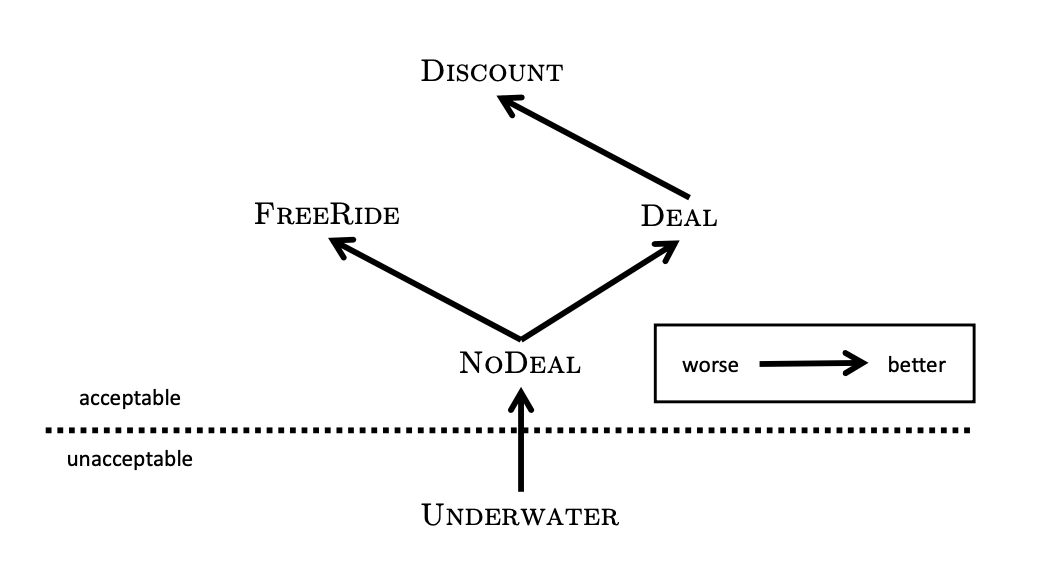
\includegraphics[width=0.8\textwidth]{figures/outcomes.png}
%     \caption{Protocol Outcomes. Figure borrowed from \cite{herlihy2018atomic}}
%     \label{fig:pro-outcome}
% \end{figure}


% Depends on the final result of the swaption, outcome of the party $p$ is categorized into following classes:
% \begin{itemize}
%     \item \textbf{FreeRide}: The party $p$ profits from the swaption by spending nothing. The benefit may include premium or some amount of punishment in the form of margin or principal.
%     \item 
% \end{itemize}




% \begin{definition}
% We call the protocol $P$ is secure for party $p$ if ... ? (Shall we explain security satisfaction in every forms of contracts ?!!)
% \end{definition}

% }
% \begin{definition}

% It should be defined exactly who and when should sign a transaction in a protocol.
% \end{definition}

        % and $tail(\hat{e}) = v_i$, then $\exists_{\hat{e} \in \hat{E}} \tau(\hat{e})=x$ and $tail(\hat{e}) = opposite(v_i)$. Then replace $v_i$ in $L$ with $opposite(v_i)$. It is clear that $L$ is still a feedback vertex set of $CG$. 
        % Next, construct the subgraph $MCG=(\dot{V}, \dot{E})$ of $CG$ by removing 
        % $\{\forall_{\hat_{v} \in \hat{V}}\}$ The locktimes of contract funding stage for each vertex is determined by the direction of $CG$ graph as descending except for the vertices in $L$.
        % opposite(v_i)$ $L'=\{v_0, v_1, .., v_{i-1}, opposite(v_i), .., v_l\}$ is another feedback vertex set of $CG$ and for vertex $opposite(v_i)$ there must exists an edge $\hat{e} \in \hat{E}$ that $\tau(\hat{e}) = x$ and $tail(e) = opposite(v_i)$, since otherwise the swaption corresponding to vertexes $v_i$ and $opposite(v_i)$ has no input from other swaptions in the $GG$ graph and the graph is no longer strongly connected.
        % Construct the subgraph $CG=(\hat{V}, \hat{E})$ of $PFG=(V, E)$ where every edges $e \in E$ that $\tau(e)$ is $t$ are removed. Assume $L=\{v_0, v_1, .., v_l\}$ is the one of the feedback vertex sets of $CG$ that for every $v_i \in L$ there is an edge $\hat{e} \in \hat{E}$ that $\tau{e} = x$ and $tail(\hat{e})=v_i$. If there is no such $L$ then there is at least one $v_i \in L$ that $\nexists_{\hat{e} \in \hat{E}} \tau(\hat{e})$ and $tail(\hat{e}) = v_i$. Then it is clear that $L'=\{v_0, v_1, .., v_{i-1}, opposite(v_i), .., v_l\}$ is another feedback vertex set of $CG$ and for vertex $opposite(v_i)$ there must exists an edge $\hat{e} \in \hat{E}$ that $\tau(\hat{e}) = x$ and $tail(e) = opposite(v_i)$, since otherwise the swaption corresponding to vertexes $v_i$ and $opposite(v_i)$ has no input from other swaptions in the $GG$ graph and the graph is no longer strongly connected. By applying this 
        % $\hat{V} = V$ and for every $\hat{e} \in \hat{E}$ 
        % that $head(e) = \hat{v_1} \in \hat{V}$ and $tail(e) = \hat{v_2} \in \hat{V}$, 
        % there is an edge $e \in E$ that $\tau(e) \in \{i, x\}$. Assume $L=(\hat{v_0}, \hat{v_1}, .., \hat{v_l})$ is the feedback vertex set of $CG$. The order of contract fundings' locktime is determined by the order of edges in the $CG$ as descending except for the vertices in $L$. The contract funding locktimes of these vertices will be in the same order but ascending. Also the parties in these vertices need to deposit margin in each of these swaptions.
        % vertex $v \in V$ where $label(v) = p_{leader}$ is determined as ascending by the order of edges in $SG=(\hat{V}, \hat{E})$ subgraph of $PFG$ where $\hat{V} = V$ and $\hat{E} = E$ that for each $\hat{e} in \hat{E}$ there is an edge $e \in E$ where $\tau(e)$ is $x$. For other parties the order is determined by the order of $PFG$ graph as ascending.
        % and for each $\hat{e} \in \hat{E}$ which $\tau{}$ 
        


    % Next, it is the \keyone key holder's turn to continue the process of contract writing by choosing his desired \keyone key. He writes the other parts of the contract up to the option Funding stage in the \depsrc swaption. The $label(opposite(\depsrc))$ party \fatemeC{note they do not need to face each other} completes her contracts up to the same stages in other swaptions where she is supposed to do it\fatemeC{where she has bought sth and she knows she is the source}\fatemeC{make an arbitrage without overlapping}
    % To continue the process of contract writing, Alice waits until all of its swaptions' contracts has been written by the other parties up to the option Funding stage. Then to finalize the contract settlement phase, Alice completes all of the contracts in her side by choosing the \Atwo key and writing the option Funding stages, and like the previous steps, everybody follows the protocol. Note that depending on the requirements of the type of each swaption, both parties sign each transaction and send each of them to their corresponding parties. For example, some transactions has to be kept by either parties, \ie~double border-colored transaction in swaption figures. In every of the above steps, if some party is asking to sign a contract with different locks than he expects, he avoids doing so and exits the contract.
    % \ahC{Mention the condition on the locks which have to be the same}
    % \ahC{all parties have to first write when they are the swaption owner, then the other swaptions}
    % Since the \keyoneGraphExtended is a directed acyclic graph and the node corresponding to the \keyone key holder is its source, there is a path from the \keyone key holder to one of the Alice's nodes, so Alice can wait until 
    % with one source
    % for other parties in her loop. Alice does this procedure sequentially beginning from genesis swaption, 
    % \ahC{since each party may have her own arbitrage tangled to Alice's swaptions, he needs to properly set the other contracts locktimes.}
    % For each swaption, Alice makes all the transactions except the Contract Funding ones. Depending on the requirements of the type of swaption, Alice and other parties sign each transaction and send each of them to their corresponding parties. For example, some transaction might be sent by either parties, \ie~double border-colored transaction in swaption figures.
    % \ahC{Note that locktimes must be set in a way that other loop owner can settle their contracts without any problem}
% \Function{whileFor}{$g_1$, $g_2$}
%     % \While{there is no $s$ that $\sigma(s)$ is $p$ and getStateOpposite($s$, $p$) is $g_1$}
%     % \State wait
%     % \EndWhile
%     \State \textbf{wait} until there is no $s$ that $\sigma(s)$ is $p$ and getStateOpposite($s$, $p$) is $g_1$
%     \For {$s$ in $V$ that $\beta(s)$ is $p$}
%     \State propose($s$, $p$, $g_2$)
%     \EndFor
%     \For {$s$ in $V$ that $\sigma(s)$ is $p$ and $InitStage[s][1] == g_1$}
%     \State propose($s$, $p$, $g_2$)
%     \EndFor
% \EndFunction
% \For{swaption $s$ that $\beta(s)$ is $p_{master}$}
        % \State propose($s$, $p_{master}$, $principal$)
        % \EndFor
% \While{there is swaption $s$ that $\beta(s)$ is $p_{master}$ and getStateOpposite($s$, $p$) is $null$}
        % \State wait
        % \EndWhile
        
        % \While{there is no swaption $s$ that $\beta(s)$ is $p_{master}$ and getState($s$, $p$) is $leader$}
        % \State wait
        % \EndWhile
% \For{swaption $s$ that $head(internalEdge(\beta(s)))$ is $p_{master}$}
        % \State propose($s$, $p_{master}$, $option$)
        % \EndFor
        % \State \textbf{for each} swaption $s$ that $head(internalEdge(\beta(s)))$ is $p$, propose($s$, $p$, $option$) 

        \\
        % \State \textbf{while} there is swaption $s$ in association set $p_{master}$ that getStateOpposite($s$, $p_{master}$) is $leader$ \textbf{wait}
        % \State \textbf{for each} swaption $s$ in the association set of $p$ \textbf{wait until} getStateOpposite($s$, $p$) = $principal$ \textbf{then} $propose(s, p_{master}, option)$
        % \While{there is swaption $s$ in association set $p_{master}$ that getState($s$, $p_{master}$) is $leader$}
        
        % that $p_{master}$ is $\beta(s)$ or $\sigma(s)$ and $InitState[s][1]$ is $leader$}
        % \State wait
        % \EndWhile
% \State \textbf{while} there is no swaption $s$ in the association set of $p$ that getStateOpposite($s, p$) is $principal$ \textbf{wait}
% \State \textbf{while} there is no swaption $s$ in the association set of $p$ that getStateOpposite($s, p$) is $option$ \textbf{wait}
        % \State \textbf{for each} swaption $s$ in the association set of $p$, propose($s$, $p_{master}$, $option$)
        % \State \textbf{for each} swaption $s$ in the association set of $p$ \textbf{wait} until getStateOpposite($s$, $p$) = $principal$ \textbf{then} $propose(s, p_{leader}, principal)$
        % \textbf{wait} until there is no swaption $s$ in the association set of $p$ that getStateOpposite($s$, $p$) is $principal$
        
        % \State $s =$ The swaption where \depsrc is in
        % \State $propose(s, p, leader)$
        % \State \textbf{for each} swaption $s$ in the association set of $p$ \textbf{wait} until getStateOpposite($s$, $p$) = $principal$ \textbf{then} $propose(s, p_{leader}, principal)$
        % \While{getStateOpposite($s$, $p_leader$) is not $principal$}
        % \State wait
        % \EndWhile
        % \State \textbf{wait} until getStateOpposite($s$, $p_{leader}$) is not $principal$
        % \State propose($s$, $p_{leader}$, $leader$)
        
        % \State whileFor($leader$, $option$)
% \State whileFor($null$, $principal$)
        % \State whileFor($principal$, $leader$)
        % \State whileFor($leader$, $option$)
% First of all, she pays all of the \textbf{Feeding Premiums} by sending \textbf{Contract Funding} trasnaction of all of her swaptions on her side. Then for each party $p$ if he gets the \textbf{Contract Funding} of his $genesis(p)$, he starts doing so on all of the swaptions in which he is its {\it Owner}. In this step, if he gets a new \textbf{Contract Funding} transaction in one of its {\it Association Set } swaptions, which he is not its owner, he follows the protocol by sending the \textbf{Contract Funding} transaction on his side. Note that in all of the mentioned steps, every party $p$ except Alice has to wait until the \textbf{Contract Funding} transactions of all of his \textbf{Association Set} swaptions except $genesis(p)$ is broadcast. Then he sends the \textbf{Contract Funding} transaction $genesis(p)$ swaption on his side. \fatemeC{why in God's name?} In this way, we can guarantee that he can settle his own deals tangled to other parties arbitrage properly. When on all of the Alice's swaptions the \textbf{Contract Funding} transactions completely broadcasted, she reveals the \Aone key on all of them and finishes the \textbf{Contract Initiation} phase. Every other parties also do the same to pass the \textbf{Contract Funding} stages in all the swaptions.
    % Then every other parties, same as the previous phase, will do the same if in all of the swaptions
    % genesis swaption on her side, then other party in genesis swaption will send his own. Afterward all parties will do the same for all of the swaptions in the order of \AtwoGraph graph. 
    % If someone in between avoids to follow the protocol, Alice will not reveal \Aone key and everything will be reverted. \ahC{needs further discussing?}
    
    
    % Note that in all of the mentioned steps, everybody except Alice has to wait until in all of the swaptions in which he is not the {\it Owner} the other party writes her own contract, then he do this step in the swaptions in which he is the owner and after getting the response on all his swaptions, he finishes this step in the swaptions which he is not their {\it Owner}. 
    
% \Function{respond}{ }
    % \For {all swaptions $s$ that $\sigma(s)$ is $p$ and $\beta(s)$ has broadcast her funding transaction}
    %     \State $p$ broadcasts her funding transaction
    %     \EndFor
    % \EndFunction
% \For {for swaptions $s$ that $\beta(s)$ is $p_{master}$}
        % \State $p_{master}$ broadcasts her funding transaction
        % \State broadcast($s, p, principal$)
% \State \textbf{for each} swaption $s$ in the associated set of $p$ 
        
        % \While{there is a swaption that has funding transactions not yet broadcast}
        % \State wait
        % \EndWhile
        % \State \textbf{for each} swaption $s$ in the associated set of $p$ \textbf{do} \tab \tab reveal($p,$ \Aone)
% \While{there is a $s$ that $\sigma(s)$ is $p$ and $s$ is a genesis swaption needing a feeding premium not yet broadcast}
        % \State wait
        % \EndWhile
% \State \textbf{wait} untill the \Aone key is reveald.
% \State \textbf{for each} swaption $s$ in the associated set of $p$ \textbf{do} \tab \tab 
% \For{all swaptions $s$} \Comment{after $p_{master}$ reveals \Aone key}
            % \If {$\sigma(s)$ is $p$ and $\beta(s)$ has revealed \Aone key}
            % \State take the premium
            % \EndIf
        
            % \If {$\beta(s)$ is $p$}
                % \State reveal \Aone key
            % \EndIf
        % \EndFor
% one of the sink nodes in of the \keyoneGraph graph. Since the \keyone key holder is the party in front of all of the sink nodes in their swaptions, he can wait until all of the parties properly deposit their principals. 
% other party's principal deposition in this swaption again, since it was proved by the lemma \ref{lm:sink} that final node in the \keyone graph hierarchy is also in the Deposition Source swaption. 
    % Now it is the \keyone key holder's turn to reveal the \keyone key following the rules which is discussed in previous sections. After all, if he avoids to reveal \keyone key, he will be punished by the rules which are mentioned before.
    % It should be noted that always the loop owner (here Alice) should 
    
        % \While{there is an input edge $e$ that $\tau(e) = x$ and $head(e)$ has not deposited}
        % \State wait
        % \EndWhile 
        % \State deposit principal
        
        % \While{$opposite(\depsrc)$ is not deposited}
        % \State wait
        % \EndWhile
        % \State reveal \keyone key
        
% \While{there is an input edge $e$ that $head(e)$ has not deposited}
        % \State wait
        % \EndWhile 
        % \State deposit principal
        
        % \State when see the \keyone revealed use it in any other swaption to get your money \fatemeC{obviously more explanation is needed}
        
        % \EndIf
        % \Comment{ mention it starts from
        % source to sink}
        
        
        
        % \State PFG is a DAG with one source and sink. Take its topological order. \fatemeC{how to say its a line?}
        % \For{vertex $v$ in the topological order}
        % \State $label(v)$ deposits her principal in $v$
        % \EndFor
        
        % \For{vertex $v$ in the topological order}
        % \State $label(v)$ reveals \keyone key
        % \EndFor
        
        % \State $p_{master}$ reveals \Atwo key. every other party does the same in a loop





% \ahC{We have to mention that all the loop owners can be considered to be Alice, because of the premium passing. }

% \begin{claim}
% Set down a claim about our newly generated lemma here dude. :)
% \end{claim}
% each party who deposit his initial asset by their own, in this graph there is a dashed-line arc from every where he is supposed to give assets in other swaptions through the flow of this money.
% his initial deposition to every where he 
% The dashed-arcs in this graph

% swaptions in the safe state. To do so, consider $s$ a swaption on $T$ which one of its outgoing arcs is triggered. Since the protocol keeps all the swaptions synchronously in one stage at a time, the swaptions corresponding to in-going arcs of $s$ are also in the same stage as $s$. Hence if $s$ is exercised, then parties in $s$ are aware of keys which opens all the locks on $s$ input arcs, then they can exercise all of them too. The parties who are responsible for keeping all the swaptions synchronously are \Atwo key holder and \keyone key holder. If one of them avoids to follow the protocol and reveals a secret before syncing a swaption, then the one who loses money is the key holder himself. If \keyone key holder reveals \keyone key before other parties principal deposition, then he donates his money without getting any. The \Atwo key holder can not reveal \Atwo key before finishing Principal Deposition phase in protocol, because still there is the \keyone key on all of the arcs and revealing the \Atwo key helps her in no way for cheating. Additionally, if \Atwo key holder and \keyone key holder try to corporately cheat on others, the early exposition of \Atwo and \keyone keys is not beneficial for \keyone key holder.
% By executing the above protocol on $T$
% \def\HS{\hspace{\fontdimen2\font}}\the\fontdimen2\font
% \begin{theorem}
% If there is a tangle $T$, then there is an algorithm $A$ which if it is executed on $T$ then the procedure for every swaption in $T$ is secure.
% \end{theorem}

% The suggested algorithm is as follows:

% % \begin{}
% \begin{itemize}
%     \item Find all the strongly connected components of \genGraph graph of $T$.
%     % \item Redo the previous line until there is no change in resulted graph.
%     \item The newly generated graph has no cycle. 
%     % Because if it has any cycle, the procedure might have continued at least one more step in the previous step. 
%     Hence there is a sequential order of components in graph. If all the components satisfy requirements mentioned in \ref{th:concurrency} theorem, then by executing protocol $P$ on all of the extracted component on this order the entire tangle can be exercised safely. 
    
% \end{itemize}
% \begin{theorem}
% \label{th:opp-gen}
% Given a tangle $T$ and all of its strongly connected components in \genGraph graph $\{c_1, c_2, ..., c_n\}$, if there is a swaption safe protocol $P$ for $T$, then every $c_i$ must be an Executable Concurrent Tangle,.
% \end{theorem}

% To prove the above theorem, we define another equivalent theorem:
% start by giving counterexample for each situation against the theorem.

% \begin{lemma}
% \label{lm:sink}
% In the \keyoneGraph graph of the concurrent tangle $T$, there is no sink node other than the \keyone key holder node in the \depsrc swaption.
% % existence of the sink nodes other than the \keyone key holder node in the 
% % \depsrc swaption is not rationally acceptable.
% \end{lemma}
% To find a desired protocol we first prove a useful lemma which will be used in the construction of our protocol:



% The situation of the swaptions that contains sink nodes in a \keyoneGraph graph can be categorized into three cases. 
% \begin{enumerate}
%     \item This is the only case that is economically justifiable. Either both parties in the swaption are not going to spend their new assets in the tangle or there is no input from other swaptions into this swaption. In both case the \genGraph of the tangle can not be in the form of \scdg, since there is no path either from this swaption to any other ones \ahC{Figure is needed} or vice versa.
%     \item The node other than the sink node in its swaption has one input. Then it is clear that the party corresponding to this node payed some asset while getting nothing in return which is economically unjustifiable.
% \end{enumerate}
% One of them which is  In the second case, 
% the sink node has no input while other one either has one output or nothing. In the first case the \genGraph graph of the tangle is no longer strongly-connected directed graph and in the second case some one in the swaption . The final case is when the swaption is the Deposition Source swaption of the tangle. By the following discussion the \ref{lm:sink} lemma is proved. As a result of this lemma, in the \keyoneGraph graph of any concurrent tangle, starting from the \keyone key holder node in the Deposition Source swaption, the final node will be the other node in the Deposition Source swaption. \ahC{Rewrite this sentence.}
% during the same phase of the execution
% then there is a swaption which has two outgoing black arcs, one arc for each of its nodes, and the locks imposed on these arcs are different.


% \ahC{We have to mention that we do not explore the case in which multiple locks are attainable for each stage}
% Then whether there is more than one source in \keyoneGraph graph or there is a cycle in \keyoneGraphExtended graph.  If there is a cycle in the \keyoneGraphExtended graph, then there is no proper way of principal deposition between the swaptions involving in the loop. In the case that there is a cycle in \keyoneGraphExtended graph, the arcs which generate the cycle can not be all black, since the money which is transferring by these arcs has no source and comes from nowhere. Additionally, if all of the arcs generating the cycle are whether dashed-arc or black arc, the only way of executing is to deviate from the order of one of the dashed-arcs. Thus certainly the party 
    % there is no proper way of executing such a cycle, since by the arguments given before, the only way of execu
    % Therefore there is at least one red arc in this cycle. Name the set of swaptions in which their red arc is the part of the cycle $\mathcal{SW}$. If there is a protocol $P$ which executes $T$, in its suggested principal deposition order there is a $sw \in \mathcal{SW}$ which its principal deposition order is by the opposit direction of its red arc. The conceivable situations of $sw$ is shown in Fig.~\ahC{Fig needed}. In both cases, the protocol is forcing one of the parties to act irrationally by the rationality property has been told in the beginning of this section. On the other words, if the threatened party can follows the rule of protocol, he is an irrational party which is not permitted in our model, and otherwise the protocol will be stopped from continuing.
    % he acts irrationally, and otherwise 
    % If $sw$ is in the shape of \ahC{Fig needed}, then the protocol forces the party $B$ to deposit his principal before $A$. Since all the parties are acting rationally by the rationality property has been told in the beginning of this section, $B$ does not provide
    % Assume there is at least two sources on the \keyoneGraphExtended graph, call these sources $src1$ and $src2$. Thus whether the \keyone locks of both sources are equal by highly unlikely chance which is impractical, or there must not be a path from the swaption corresponding to the $src1$ node to the swaption of the $src2$ node, the \genGraph graph of tangle at least has two separately components which contradicts with the \scdg property of it. Otherwise there is a swaption tangle which the \keyone locks on its black arcs are not the same and it is probable for one of its parties to  enter the \textbf{Underwater} state.
% Since the \genGraph of $c_i$ is strongly connected, then all of the swaptions in the $c_i$ are locked by multiple \keyone locks if there is more than one source on graph, and these locks will be equal by highly unlikely chance which is impractical. Additionally, if there is a cycle in the \keyoneGraph graph, then there is no proper order of principal deposition for the nodes inside the cycle, thus no such a protocol can suitably exercise the case.
    % needed to have multiple \keyone lock which is not in permited in the definition of our problem.
% defiantly there is some person which during the execution of tangle do not understand the \Atwo 
    % who has a mother vertex in the \genGraph graph. Then the locks on black arcs in the \AtwoGraph graph of $T$ may differ which each other since there is no party responsible to impose a similar lock on all the arcs. Finally by imposing different \Atwo locks, like the argument for previous case, this is also impossible that all the \Atwo locks are the same and there might be a swaption which exits the safe secure state.
    % there are parties and nodes in $T$ the one who has the opening key for \Atwo lock
    % either there is no winner candidate of the tournament, which tells us there is no party eligible to be the \Atwo key holder of the tangle to tell every body the opening key of \Atwo lock. 
    % Then either there is more than one Owner for tangle, which like previous argument about multi \keyone locks this case is also practically impossible, or there is no mother vertex in the \genGraph graph corresponding to the unique owner
    % Then there is more than one party which acts as the Mother vertex of tangle. Exactly like the argument for previous case, this is also impossible that all the \Atwo locks are the same.
    % either no {\it Main Loop} in $c_i$, so no \Atwo lock is used, hence there is no option, or there is at least two loops which do not have same owners. Like the argument in previous situation, in this case there is a swaption in which multiple \Atwo keys are used which is not attainable in our model.
    % \item $c_i$ is not {\it Startable}: 

% \begin{definition}{Concurrent Executable}
% A concurrent tangle is Concurrent Executable if it is {\it Startable} and {\it \AtwoGraph Acceptable} and {\keyoneGraph Acceptable}.
% \end{definition}

% Given a tangle $T$ and all of its strongly connected components in \genGraph graph $\{c_1, c_2, ..., c_n\}$, if every $c_i$ is Executable Concurrent Tangle, then there is a protocol $P$ which if it is executed on $T$ then the procedure for every swaption in $T$ is secure.

% A protocol $P$ for a swaption $s$ is secure if during the execution of $P$ on $s$ any outgoing arc is triggered from $s$, then every ingoing arcs also will be triggered.
% \ahC{Is really this security property fits to what we want? Each parties asset is the input of other, shall we define in a better way?}
% If there is an Executable Concurrent tangle $T$, then there is a protocol $P$ which is tangle secure for $T$.
% is secure for each party participating in $T$. 
% the only sink vertices is the $opposite(\text{\depsrc})$ of the graph.

% there is no sink node other than the node in front of 
% \keyone key holder node in the Deposition Source swaption is not rationally acceptable.
% Assume the \keyoneGraph graph of $T$ is $PFG=(V, E)$, and 
% \begin{itemize}
%     \item $\exists_{e \in E \and \tau(e)=x} head(e)=opposite(s)$: 
%     \item otherwise: 
% \end{itemize}
% , whether there is an edge $e$ which $\tau(e)=e$ and $head(e)=opposite(s)$ or not. 
% The conceivable shapes of the corresponding swaption of $sw$ are shown in Fig.~\ref{fig:sink-shapes}.
% As it is shown in figures, the node other than $s$ in its swaption, name this node as $f$, must have an outgoing arc, since otherwise there is no path from this swaption to any other swaption and the form of the \genGraph of $T$ is no longer \scdg.
% If this node does not have an ingoing arc, $f$ is the source of graph, hence $s$ is the {\it Final Node } of the tangle which does not contradicts the lemma.
% Therefore the only possible shape is in the form of Fig.\ref{fig:sink-2}. By the properties of the \keyoneGraphExtended, the right hand side label of the swaption $sw_0$ has to be $B$, since the output money of $A$ in $s$ belongs to the party $B$. Also, we can say that the left hand side label on swaption $sw_1$ is $A$. Since the party $A$ does not spend her money in $s$, she is forming a line of swaptions in which she deposits the initial money from her own. One may claim that the party $A$ formed a series of swaptions in the form of Fig.\ref{fig:sink-3}. By analysing the situation of the {\it conjunction swaption } in this graph, whether this swaption is between $A$ and $A$ which does not make any sense, or one of its nodes has multiple black outgoing arc that is not allowed in our model. Therefore, the party $A$ forms a line of swaptions in the form of the Fig.\ref{fig:sink-2}. In the beginning swaption of this line, $A$ deposits her principal from her own, hence there is node in this swaption labeled by $A$ that has not any ingoing black arc. Therefore there must be a dashed-arc between $s$ to this node. Thus $s$ is no longer sink node.
% All in all, the only allowable sink node in a concurrent tangle is the $opposite(\text{\depsrc})$ of the tangle.
% the red arc of the swaption must be destined to $s$, otherwise 
% The situation of the swaptions of sink nodes in a \keyoneGraph graph can be categorized into three cases. One of them which is economically justifiable is when both parties in the swaption are not going to spend their new assets in the tangle. In this case the \genGraph of the tangle can not be in the form of strongly-connected directed graph, since there is no path from this swaption to any other ones \ahC{Figure is needed}. In the second case, the sink node has no output while other one either has one output or nothing. In the first case the \genGraph graph of the tangle is no longer strongly-connected directed graph and in the second case some one in the swaption payed some asset while getting nothing in return which is economically unjustifiable. The final case is when the swaption is the Deposition Source swaption of the tangle. By the following discussion the \ref{lm:sink} lemma is proved. As a result of this lemma, in the \keyoneGraph graph of any concurrent tangle, starting from the \keyone key holder node in the Deposition Source swaption, the final node will be the other node in the Deposition Source swaption. \ahC{Rewrite this sentence.}
% For convenient reason, we assume that our tangle only has one {\it Arbitrage Owner}, called Alice, and she is 
   % In the beginning of the procedure she does not know the hash of the \keyone key. Hence she only can write contracts for her opponents up to the leader lock stage. 
    % In this step every other party that this contract has been written for does the same as Alice for their own swaptions. 
        % For every edges $e \in E$ that $head(e)=v_h$ and $tail(e)=v_t$ and $\tau(e)$ is $x$, there is an edge $\hat{e} \in \hat{E}$ that $tail(\hat{e}) = \hat{v_t}$ and $head(\hat{e}) = \hat{v_h}$. Also, for every edges $e \in E$ that $head(e)=v_h$ and $tail(e)=v_t$ and $\tau(e) = i$, there is an edge $\hat{e} \in \hat{E}$ that $tail(\hat{e}) = \hat{v_h}$ and $head(\hat{e}) = \hat{v_t}$.
        % \ahC{Nice fact, but useless :(}Construct the subgraph $CG=(\hat{V}, \hat{E})$ of $PFG=(V, E)$ where every edges $e \in E$ that $\tau(e)$ is $t$ are removed. Assume $L=\{v_0, v_1, .., v_l\}$ is the feedback vertex sets of $CG$. 